\documentclass[12pt,a4paper]{article}
\usepackage{amsmath,amscd,amsbsy,amssymb,latexsym,url,bm,amsthm}
\usepackage{epsfig,graphicx,subfigure}
\usepackage{enumitem,balance}
\usepackage{wrapfig}
\usepackage{mathrsfs,euscript}
\usepackage[usenames]{xcolor}
\usepackage{hyperref}
\usepackage[vlined,ruled,linesnumbered]{algorithm2e}
\usepackage{array}
\hypersetup{colorlinks=true,linkcolor=black}

\newtheorem{theorem}{Theorem}
\newtheorem{lemma}[theorem]{Lemma}
\newtheorem{proposition}[theorem]{Proposition}
\newtheorem{corollary}[theorem]{Corollary}
\newtheorem{exercise}{Exercise}
\newtheorem*{solution}{Solution}
\newtheorem{definition}{Definition}
\theoremstyle{definition}

\renewcommand{\thefootnote}{\fnsymbol{footnote}}

\newcommand{\postscript}[2]
 {\setlength{\epsfxsize}{#2\hsize}
  \centerline{\epsfbox{#1}}}

\renewcommand{\baselinestretch}{1.0}

\setlength{\oddsidemargin}{-0.365in}
\setlength{\evensidemargin}{-0.365in}
\setlength{\topmargin}{-0.3in}
\setlength{\headheight}{0in}
\setlength{\headsep}{0in}
\setlength{\textheight}{10.1in}
\setlength{\textwidth}{7in}
\makeatletter \renewenvironment{proof}[1][Proof] {\par\pushQED{\qed}\normalfont\topsep6\p@\@plus6\p@\relax\trivlist\item[\hskip\labelsep\bfseries#1\@addpunct{.}]\ignorespaces}{\popQED\endtrivlist\@endpefalse} \makeatother
\makeatletter
\renewenvironment{solution}[1][Solution] {\par\pushQED{\qed}\normalfont\topsep6\p@\@plus6\p@\relax\trivlist\item[\hskip\labelsep\bfseries#1\@addpunct{.}]\ignorespaces}{\popQED\endtrivlist\@endpefalse} \makeatother

\begin{document}
\noindent

%========================================================================
\noindent\framebox[\linewidth]{\shortstack[c]{
\Large{\textbf{Lab07-Amortized Analysis}}\vspace{1mm}\\
CS214-Algorithm and Complexity, Xiaofeng Gao, Spring 2020.}}
\begin{center}
\footnotesize{\color{red}$*$ If there is any problem, please contact TA Shuodian Yu. }

\footnotesize{\color{blue}$*$ Name: Yulong Hui  \quad Student ID: 518030910059 \quad Email: qinchuanhuiyulong@sjtu.edu.cn}
\end{center}
\begin{enumerate}
	\item For the TABLE-DELETE Operation in Dynamic Tables, suppose we construct a table by multiplying its size by $\frac 23$ when the load factor drops below $\frac 13$. Using \emph{Potential Method} to prove that the amortized cost of a TABLE-DELETE that uses this strategy is bounded above by a constant.
	
	\begin{solution}
		~\\
		First we define load factor $\alpha(T)$, which means the quotient of the $num_t$ and $size_t$.
		 
		Then, We can start by defining a potential function $\Phi(T) $ that is 0 immediately after a contraction, and builds as $\alpha(T) $ decreases to $\frac{1}{3} $
		$$\Phi(T)=size_t-num_t $$
		
		\textbf{Correctness}: The potential is 0 for an empty table, and $\Phi(T)$ never goes negative. Thus, the total amortized cost of a sequence of $n$ operations with respect to $\Phi$ is a upper bound of the actual cost.
		
		Then, let $ C_i $ means the complexity of i-th delete-operation, and define:
		$$ \widehat{C_i}=C_i+\Phi(i)-\Phi(i-1)$$
		
	   \textbf{Case 1:} $\alpha(i-1)>\frac{1}{3}$, and there is no contraction.
	     
		
		 \begin{equation}\nonumber
		 \begin{aligned}
		 \widehat{C_i}&=C_i+\Phi(i)-\Phi(i-1)
		 \\&=1+size_i-num_i-(size_{i-1}-num_{i-1})
		  \\&=1-(num_{i-1}-1)+num_{i-1}
		  \\&=2
		 \end{aligned}
		 \end{equation}
		 
		  \textbf{Case 2:} $\alpha(i-1)=\frac{1}{3}$, and there is a contraction.
		 
		 
		 \begin{equation}\nonumber
		 \begin{aligned}
		 \widehat{C_i}&=C_i+\Phi(i)-\Phi(i-1)
		 \\&=1+num_i+ size_i-num_i-(size_{i-1}-num_{i-1})
		 \\&=num_{i-1}+\frac{2}{3}\times size_{i-1}-(num_{i-1}-1)-size_{i-1}+num_{i-1}
		 \\&=num_{i-1}+\frac{2}{3}\times 3\times num_{i-1}-num_{i-1}+1-3\times num_{i-1}+num_{i-1}
		 \\&=1
		 \end{aligned}
		 \end{equation}
		
		Therefore, we can get:
		$$\sum_{i=1}^{n}{C_i}\leq  \sum_{i=1}^{n}\widehat{C_i}<2n=n\times O(1) $$				
		
		Then we can say: the amortized cost of a TABLE-DELETE is bound above by a constant.
		
	\end{solution}
	

	
	\item A \textbf{multistack} consists of an infinite series of stacks $S_0, S_1, S_2,\cdots$, where the $i^{th}$ stack $S_i$ can hold up to $3^i$ elements. Whenever a user attempts to push an element onto any full stack $S_i$, we first pop all the elements off $S_i$ and push them onto stack $S_{i+1}$ to make room. (Thus, if $S_{i+1}$ is already full, we first recursively move all its members to $S_{i+2}$ .) An illustrative example is shown in Figure \ref{Fig-MultiStack}. Moving a single element from one stack to the next takes $O(1)$ time. If we push a new element, \underline{we always intend to push it in stack $S_0$}.

	\begin{figure}[!htbp]
	\centering
	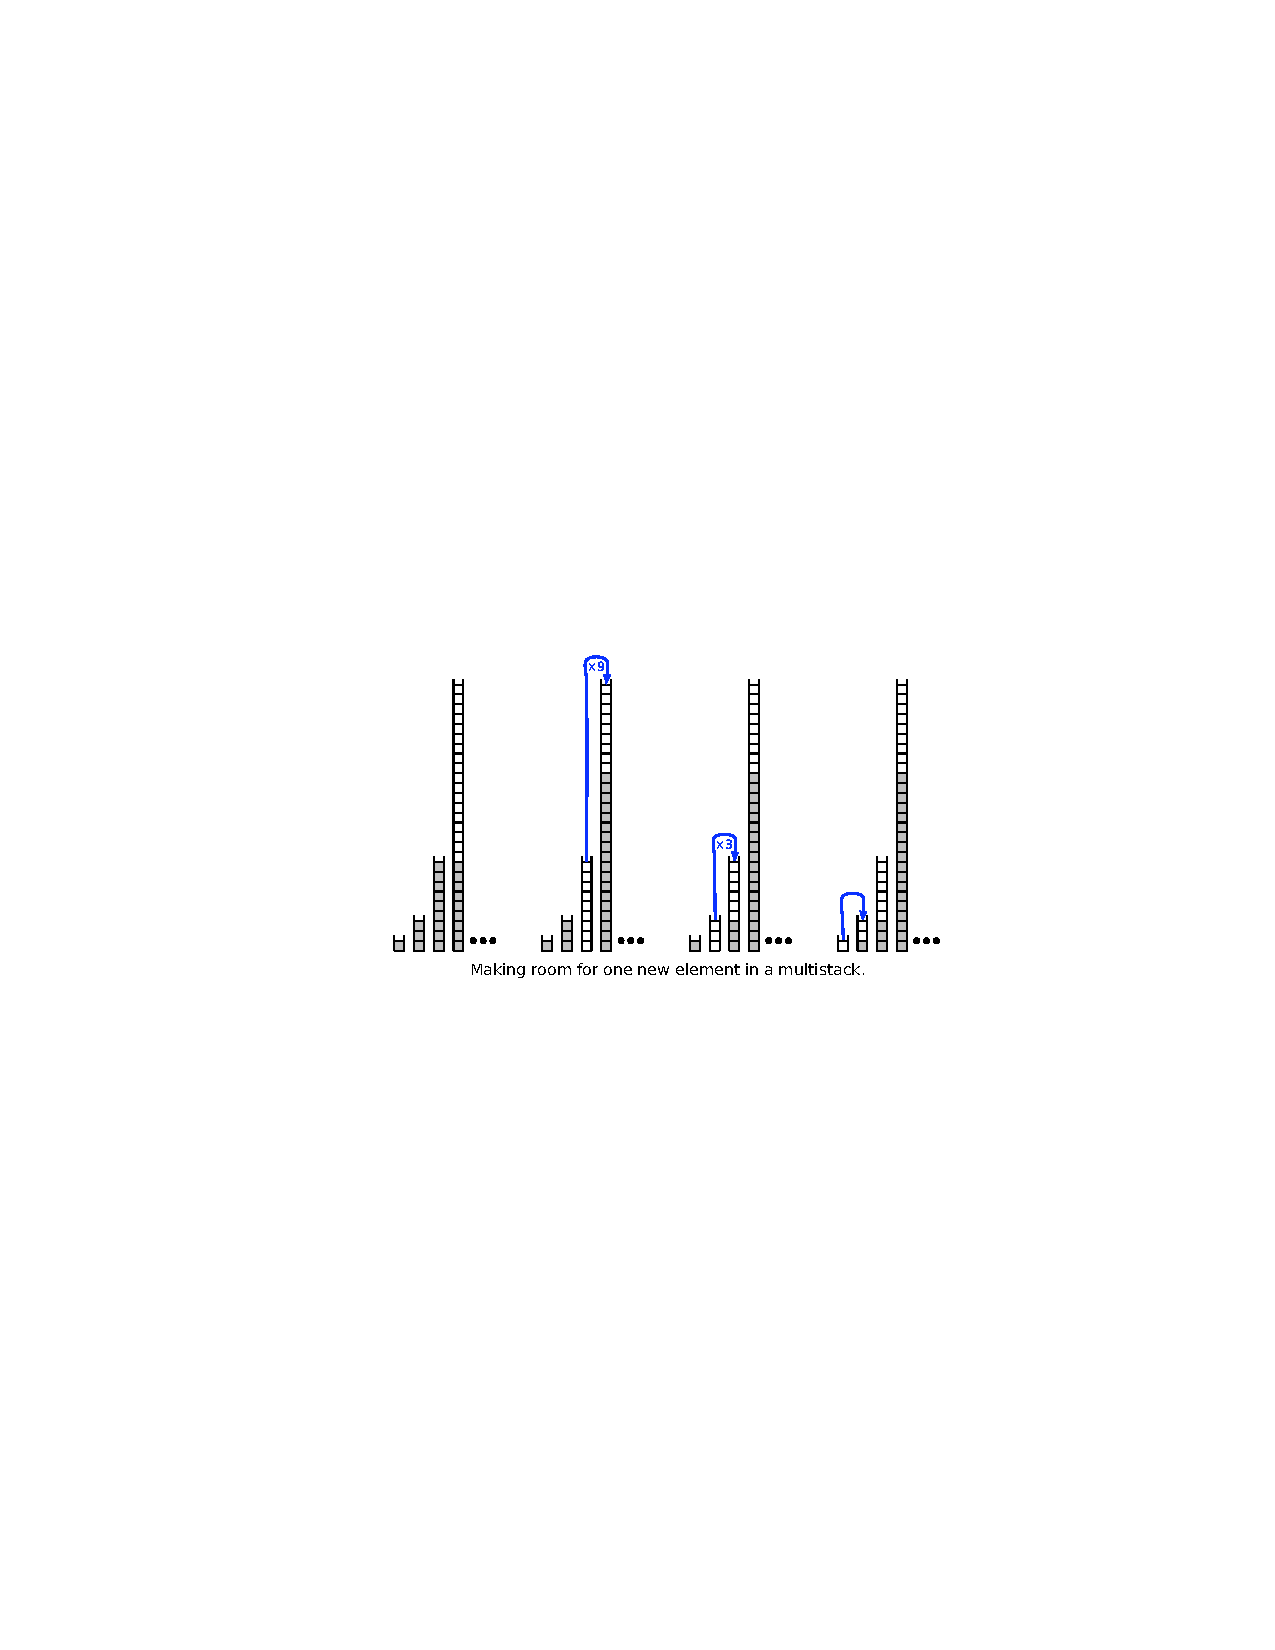
\includegraphics[width=0.4\textwidth]{Fig-MultiStack.pdf}
	\caption{An example of making room for one new element in a multistack.}
	\label{Fig-MultiStack}
	\end{figure}

    \begin{enumerate}
        \item In the worst case, how long does it take to push a new element onto a multistack containing $n$ elements?
        \item Prove that the amortized cost of a push operation is $O(\log n)$ by \emph{Aggregation Analysis}.
        \item {\color{red}(Optional Subquestion with Bonus)} Prove that the amortized cost of a push operation is $O(\log n)$ by \emph{Potential Method}.
    \end{enumerate}
	
	~\\
	\textbf{Solution.}
	
	\begin{enumerate}
		\item In the worst case, all of the used stack is full, which means we should pop and push all of the existing elements. 
		
		Since moving single element needs $O(1)$ time, in the worst case:  $$(n+1)*O(1)=O(n)$$
		Therefore, we need $O(n)$ time.
		\item First, calculate the sequence of operation-numbers, when we push new element continuously:
		\begin{figure}[!htbp]
			\centering
			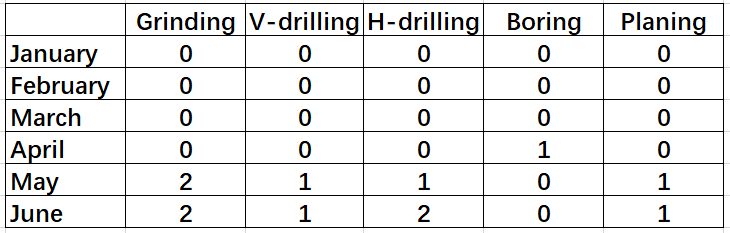
\includegraphics[width=0.35\textwidth]{1.png}
			\caption{The procedure of pushing new element}
			\label{Fig-MultiStack}
		\end{figure}
	
		In the figure above, every row represents the number of  existing elements in $S0,S1,S2,S3$ (the first row means there are no element at first). 
		
		The value of "OP" means the operation-number at the corresponding stage.
		
		The right column explains the composition of every operation-number.
		
		As you can see, every time the i-th stack is full, we should move its elements, so the operation-number should add $3^i$, and we can say $S_i$ conributes $3^i$ to the OP.
		
		~\\
		Then, consider pushing $ n$ elements.
		
		For $S1$, it needs $(1+3)$ element-pushing to get full at first, then it will get full every 3 pushings. So the total contribution of $S1$ is less than $3\times \frac{n}{3}=n$
		
		
		The same to others, $S_i$ needs $(1+3+9+...+3^i)$ element-pushing to get full at first, then it will get full every $i$ pushing.  So the contribution of $S_i$ is less than $3^i\times \frac{n}{3^i}=n$
		
		Then,  we just need $j$ stacks to hold $n$ elements,so the total operation number can be:
		$$OP_{total}=Contribution(S_0)+Contribution(S_1)+....+Contribution(S_j)$$
		$$OP_{total}<n+n+n+...+n=j*n$$
		
		About $j$, we can get:
		$$3^0+3^1+3^2+...+3^j \geq n \geq 3^0+3^1+3^2+...+3^{j-1}$$
		$$\frac{1-3^{j+1}}{1-3} \geq n \geq \frac{1-3^j}{1-3}$$
		$$j =[ \log_{3} {(2n+1)}]$$
		
		Therefore$$OP_{total}<n\times j =n\times [ \log_{3} {(2n+1)}]=O(n\log n)$$ The amortized cost is $O(\log n)$
		
		
		\item After the i-th pushing, we can define $ele_{i,j}$, which means the number  of elements that are held in the stack $S_j$ after i-th pushing.
		
		For example, if $i=13$, the stacks respectively hold: 9,3,1. Then, $ele_{13,0}=1$, $ele_{13,1}=3$, $ele_{13,2}=9$. Besides, the largest stack number (in this case, is $2$) is defined as $t$.
				
		Define $\Phi(i)$ and $\widehat{C_i}$ :		
		$$\Phi(i)=\sum_{j=0}^{t}ele_{i,j}\times(\log_3 (2n+1)-j  )$$
		
		%Then, consider any $i$, if it has \textbf{continuous} full stacks of number $m$, then we must move all elements in these $m$ stacks at the next pushing. So $C_i=1+3^0+3^1+..+3^m$
		
		$$\widehat{C_i}=C_i+\Phi(i)-\Phi(i-1) $$	
		
		\textbf{Correctness.} It's easy to see when $i=0$, $\Phi(0)=0$.
		Then, we have calculated: $j =[ \log_{3} {(2n+1)}]$ in (b).
		So $\log_{3} {(2n+1)}\geq j$, then we can get: $\Phi(i)\geq 0$ and $$\sum_{i=1}^{n}{C_i}\leq  \sum_{i=1}^{n}\widehat{C_i}$$
		
	
		
		For convenience, we let $\log_3 (2n+1)=A$
		
		
			$$\widehat{C_i}=C_i+\Phi(i)-\Phi(i-1) $$
			$$\widehat{C_i}=C_i+\sum_{j=0}^{t}ele_{i,j}\times(A-j)-\sum_{j=0}^{t'}ele_{i-1,j}\times(A-j)$$
		$$\widehat{C_i}=C_i+\sum_{j=0}^{t}ele_{i,j}\times A-\sum_{j=0}^{t'}ele_{i-1,j}\times A - (\sum_{j=0}^{t}ele_{i,j}\times j-\sum_{j=0}^{t'}ele_{i-1,j}\times j )$$
		After the i-th pushing, the total number of elements will increase by one, then  we get:
		
			$$\widehat{C_i}=C_i+ A - (\sum_{j=0}^{t}ele_{i,j}\times j-\sum_{j=0}^{t'}ele_{i-1,j}\times j )$$
		
		If there  are \textbf{ k movements} before the pushing, then we will get:
		$$C_i=1+3^0+3^1+..+3^{k-1}$$
		Because there is no movement to $S_{k+1},S_{k+2}..$ stacks, we can know: 
		
		$ele_{i,k+1}=ele_{i-1,k+1} \text{ and } ele_{i,k+2}=ele_{i-1,k+2}....$ then we can extend the formula and  get: 
		$$\sum_{j=0}^{t}ele_{i,j}\times j-\sum_{j=0}^{t'}ele_{i-1,j}\times j = 3^0+3^1+..+3^{k-1}  $$
		
		
		
		 $$C_i=1+\sum_{j=0}^{t}ele_{i,j}\times j-\sum_{j=0}^{t'}ele_{i-1,j}\times j $$
		$$\widehat{C_i}=1+A=O(\log_3(2n+1))=O(\log n) $$
		
	 $$\sum_{i=1}^{n}{C_i}\leq  \sum_{i=1}^{n}\widehat{C_i}=O(n\log n)$$
		Finally, we get the amortized cost is $O(\log n)$
		

		
		
		
		
		
	\end{enumerate}
	

	
	
	
	
	\item Given a graph $G = (V, E)$, and let $V'$ be a strict subset of $V$. Prove the following propositions.
	
	\begin{enumerate}
		\item Let $T$ be a minimum spanning tree of a $G$. Let $T'$ be the subgraph of $T$ induced by $V'$, and let $G'$ be the subgraph of $G$ induced by $V'$. Then $T'$ is a minimum spanning tree of $G'$ if $T'$ is connected.
		\item Let $e$ be a minimum weight edge which connects $V'$ and $V \setminus V'$. There exists a minimum weight spanning tree which contains e.
	\end{enumerate}

	~\\
	\textbf{Proof.}
	
	\begin{enumerate}
		\item Assume there is $n$ vertices in $T$, then the number of edges should be $n-1$. We can arrange the deleting procedure: when we induce some vertices in T, we should do deletion one by one from low degree to high degree. It's easy to see this procedure will not change the result.
		
		Then, if $T'$ is connected, it requires: each node we delete must be leaf node with degree of 1 .
		
		We can prove above statement by contradiction, if we induce a node with degree more than one, then we will lose 2 or more edges and there may be $(i-3)$ or less edges  with $(i-1)$ vertices which can not be connected. So, we can only induce the leaf node.
		
		Then it is easy to see, if we only induce a leaf node, the graph $G$ will lose a vertex and all egdes on it, while the $T$ will just lose that vertex and one edge, so it remains to be a minimum spanning. Because it still connects  all of the $n'$ nodes in graph with $n'-1$ edges, and these edges are inherited from the last minimum spanning tree, which ensures the minimum weight.
				
		We can do the above induction for several times and get $G'$ and $T'$ (each time delete one leaf node), then $T'$ must be a minimum spanning tree of $G'$.
		
	   \item Obviously, there must exist a minimum weight spanning tree callde $T$. We only need to prove $T$ contains $e$  by contradiction-method.
	   
	   Assume that the minimum spanning tree $T$ excludes this minimum weight edge $(u_0,v_0)$ (which is also expressed as $e$), and the $V'$ and $V/ V'$ are connected by  edge $(u_1,v_1)$. 
	   
	   If we add the edge $(u_0,v_0)$ to the tree $T$, then there will be a circle which passes through: $ u_0,v_0,u_1,v_1$. We can delete any one of the edges among this vertices to get a new spanning tree. We choose to delete $(u_1,v_1)$ and remain $(u_0,v_0) $, and  because weight of $(u_1,v_1)$ is replaced by a less one , the new tree is smaller than the used-defined minmum spanning tree, which means a contradiction.
	   
	   Therefore, the assumption is proved to be false, and the minmum spanning tree must include the minimum edge $(u_0,v_0)$ (which can also be expressed as $e$).
	    
		
	\end{enumerate}
\end{enumerate}



\textbf{Remark:} Please include your .pdf, .tex files for uploading with standard file names.


%========================================================================
\end{document}
